\documentclass[10pt,a4paper]{article}
\usepackage[latin1]{inputenc}
\usepackage{amsmath}
\usepackage{amsfonts}
\usepackage{amssymb}
\usepackage{graphicx}
%\usepackage{bbding}
%\ScissorHollowRight

\usepackage{amsthm} % newtheorem
\newtheorem{pb}{Problem}
\newtheorem{theoreme}{Theorem}
\theoremstyle{definition}
\newtheorem{defi}{Definition}
\newtheorem{lemma}{Lemma}
\theoremstyle{remark}
\newtheorem{rem}{Remark}

\renewcommand{\textbf}[1]{\begingroup\bfseries\mathversion{bold}#1\endgroup}
\newcommand{\fin}{\begin{flushright}
$\Box$
\end{flushright}}

\usepackage{hyperref}
\hypersetup{colorlinks,citecolor=red,filecolor=blue,linkcolor=blue,urlcolor=blue}

\usepackage[ruled,vlined]{algorithm2e}
\SetKwInOut{Input}{Input}\SetKwInOut{Output}{Output}

\newcommand{\V}{$\mathbb{V}$}
\newcommand{\D}[1]{$\partial$#1}
\newcommand{\C}{$\mathcal{C}$}
\renewcommand{\L}{$\gamma$}
\renewcommand{\S}{$\mathbb{S}$}
\newcommand{\Dual}{$G^*$}
\newcommand{\DualAdj}{$\overline{G^*}$}
\newcommand{\Ciz}{ciz}
\newcommand{\Sys}{$\mathcal{Y}$}
\newcommand{\PbOne}{1-MIN-CUTTING}
\newcommand{\PbTwo}{2-MIN-CUTTING}
\renewcommand{\P}{$\mathbb{P}$}
\newcommand{\K}{$\mathcal{K}$}
\newcommand{\MinC}{\C$_{min}$}
\newcommand{\N}[1]{$\mathcal{N}_{\textnormal{#1}}$}
\newcommand{\Ns}[1]{\D{\N{#1}}}
\newcommand{\Path}{$\mathcal{P}$}
\newcommand{\Cut}[2]{scissor(#1, #2)}

\author{Quentin Fortier}
\title{Graph-based models of volumetric medical data and applications to topological correction}
\begin{document}
\maketitle
\tableofcontents
Todo: Ex ENS, diff tetgen -q, precalculer BFS pour optimize all

\begin{abstract}
After stating some results about surface cutting, this article gives an algorithm to "optimally" cut a volume, based on pants decomposition, and several variants. It introduces two new algorithms, the neighborhood algorithm and the single path algorithm, and a C++ code named OC3D, which are my main contributions. 
\end{abstract}

\section{Introduction}
The reader not familiar with basic algebraic topology will find in the appendix the definitions needed in this report.
\subsection{Overview}
The limited resolution or the noise may increase the genus of the surfaces given by medical images and
we want to remove them, both to have a more accurate image and apply algorithms that need genus 0 surfaces. \\
For that purpose, important works have been done in finding the shortest system of loops cutting reducing the genus to 0: several methods were proposed, for example in \cite{JMThese} or \cite{EricThese}. \\
The goal of this internship is to extend these methods to a volumic topological correction, in which only few works have been done. \\

\subsection{Modelling}
For more precision, we first need some definitions: (all surfaces are assumed to be closed)

\begin{defi}
A \textit{volume} \V{} (resp. \textit{surface}) is a topological 3(resp. 2)-manifold.
We assume a volume has one boundary \D{\V} and the genus g of \V{} (i.e the genus of \D{\V}) is assumed to be different from 0.
\end{defi}

From an algorithmic point of view, instead of an abstract 3-manifold we deal with either a 3-mesh (a set of tetrahedra) or voxels, which are obviously a volume in the sense of the above definition. We will refer to them as discrete volume. Discrete surfaces are either sets of triangles or of faces of a voxel set.\\
Moreover, we assume these discrete volumes or surfaces to have a weight on their faces or edges (typically, the weight will be the length for an edge and the area for a face or the probability that the two volumic elements are adjacent, given by the segmentation step). \\

\begin{figure}[htb]
  \begin{center}
    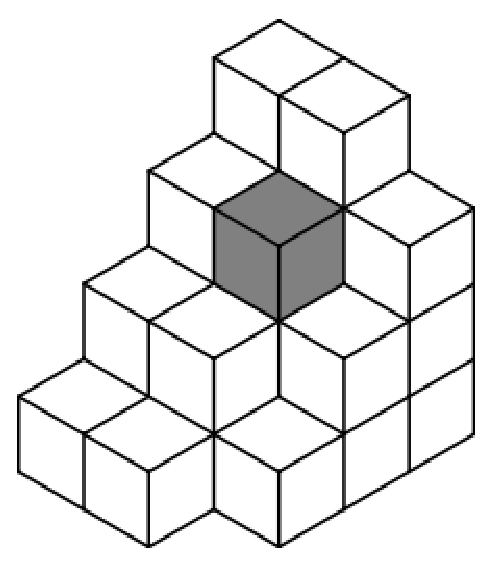
\includegraphics[height=2cm]{voxels.eps}
    \caption{Voxels}
  \end{center}
\end{figure}

\begin{defi}
Given a discrete volume \V, the \textit{dual graph} \Dual{} = (V, E) of \V{} is contructed the following way:
\begin{itemize}
\item The vertices of \Dual{} are the volumic elements (tetrahedra or voxels).
\item Two vertices are connected if the corresponding two elementary volumes share a face, and the weight of this edge is the weight of the face.
\end{itemize}
Two edges of \Dual{} are adjacent if the corresponding faces share an edge of \V{}.
\end{defi}

Since every edge in \Dual{} has a degree at most d, with d =  6 if \V{} is a voxel set and d = 4 if \V{} is a 3-mesh, 2 E = $\sum deg(v)$ $\leqslant$ d V, so O(E) = O(V).

\begin{defi}
Let A, B be two sets such that A $\subset$ B and B is connected. \\
A is B-\textit{non-separating} if B - A is connected. \\
Similarly, if $A_i$ $\subset$ B, $\lbrace A_1, \ldots, A_n \rbrace$ is B-non-separating if B - $\bigcup$ $A_i$ is connected.
\end{defi}

\begin{defi}
A \textit{1-cut} \L{} (on a surface \S{}) is a \S{}-non-separating loop.
\end{defi}

On \Dual{}, a 1-cut is a simple cycle of edges.
\begin{rem}
A contractible loop is always separating, but the converse is false. [cylinder]
\end{rem}

\begin{defi}
A \textit{2-cut} \C{} (in \V{}) is a connected, \V{}-non-separating, genus-0 surface such that \D{\C} lies on \D{\V}.
\end{defi}

On \Dual{}, a 2-cut is a set of adjacent edges (however it is not sufficient, since we require the set to be a manifold).

\begin{defi}
The \textit{cutting product} of a surface along a 1-cut \L{} is, informally, the surface produced by duplicating every edge and vertex and removing the adjacences between faces sharing an edge in \L{}. \\
The informal definition is similar for a volume. \\
See \cite{JMThese}, p. 35, for a more precise definition.
\end{defi}

\begin{defi}
A \textit{system of} 2(resp. 1)-\textit{cuts} of \V{} (resp. \S) is a \V{}(resp. \S{})-non-separating set of 2(resp. 1)-cuts such that the resulting cutting product has genus 0 and every pair of cuts doesn't intersect. 
\end{defi}

We can now give the main issue of this report: 
\begin{pb} [\PbTwo]
Given a discrete volume \V, find a minimum system of 2-cuts. 
\end{pb}

We are also interested in the related problem on surface, which we will investigate first:
\begin{pb} [\PbOne]
Given a discrete surface \S, find a minimum system of 1-cuts. 
\end{pb}
These minimums exist: there are finitely many sets of g 1-cuts (resp. 2-cuts).

\subsection{NP-hardness}
An apparently similar problem is known to be NP-hard: \\
\begin{pb} [\PbOne -BOUNDARY]
Given a discrete surface \S, possibly with boundary, find a minimum cutting to obtain a single topological disk (i.e the resulting cutting product must have genus 0 and with no boundary).
\end{pb}

\begin{theoreme}
\PbOne -BOUNDARY is NP-hard
\end{theoreme}
\textit{Proof}:~~ \\
\cite{Erickson02} reduces this problem to the \textit{rectilinear Steiner tree problem} (i.e,  given n points in the plane, find a tree connecting them all with only vertical and horizontal line segments), which is known to be NP-hard.
\fin

However, it is not known if \PbOne{} and \PbTwo{} are NP-hard, but the two problems are linked. \\
In the case of voxels, we have:
\begin{theoreme}
\PbOne{} reduces to \PbTwo.
\end{theoreme}
\textit{Proof}:~~ \\
Let \S{} be an instance of \PbOne: according to Jordan's theorem, \S{} bounds only one volume \V. \\
For each face of \V, we put a weight equals to sum of weights of the edges of this face that are in \S. 
This way the area of a surface in \V{} equals its perimeter. \\
The size of \V{} is polynomial in the size of \S{} according to the isoperimetric inequality: 36 $\pi$ vol(\V)$^2$ $\leqslant$ area(\S)$^3$, and since the volume of \V{} equals the number of voxels in \V, the area of \S{} equals the number of faces (squares) in \S.
\fin
The same theorem holds for tetrahedra if we restrict the problem to PLC (\textit{piecewise linear complex}) which can be tetrahedrized (not all surfaces can be tetrahedrized).
\subsection{Relations between the two problems}
Although they have similarities, the two problems above are not identicals and especially, minimizing the area of a surface is not equivalent to minimizing its perimeter. \\
Moreover, a surface with bounded area may have a perimeter equals to infinity.\\

\begin{figure}[h]
\begin{center}
\begin{minipage}{0.4\linewidth}
\centering 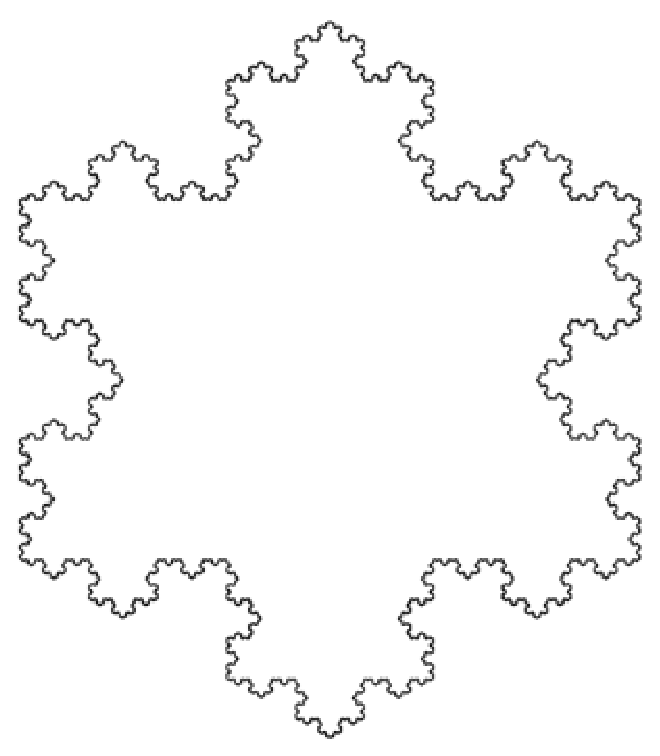
\includegraphics[height=2cm]{koch_snowflake.eps}
\end{minipage}
\hfill
\begin{minipage}{0.4\linewidth}
\centering \includegraphics[height=2cm]{torus_star.eps}
\end{minipage}
\caption{Left: The Koch snowflake, a surface with finite area but with infinite perimeter. 
Right: The optimal 1-cut (in blue) is different from the optimal 2-cut (in red) of this torus. }
\end{center}
\end{figure}
\section{Previous works on surface cutting}
In all this section, let \S{} be a surface with genus g.\\
This section introduce two algorithms dealing with \textbf{surface cutting}, the first described in \cite{JMThese}, chap. 3 and the second in \cite{EricThese}, chap. 3.\\
Both use a similar approach to find 1-cuts: they first show that computing a 1-cut is easy if we add constraints to it and then they split the surface, to force the wanted constraints.

\subsection{Cutting a surface to reduce its genus to 0}

Using the following approach, we can get a good approximation of a minimum system of 1-cuts of \S.
\begin{lemma}
We can calculate the shortest 1-cut on \S{} passing through a fixed point p in O(Vlog(V)).
\end{lemma}
\textit{Proof}:~~ \\
We use Dijkstra's algorithm from p. As soon as we meet a vertex previously visited, we look at the number c of connected components of the complementary of the surface: if c equals one we continue our search, otherwise (c equals two) we found a shortest 1-cut from p.
\fin
\begin{lemma}
We can compute a first system of 1-cut \Sys{} on \S{} in O(V).
\end{lemma}
\textit{Proof}:~~ \\
Let t be a volumic element (triangle). We use the \textit{cut locus} associated to t, i.e the the set of all points having more than one shortest path from t. 
\fin
\begin{lemma}
Every 1-cut of \S{} crosses \Sys.
\end{lemma}
\textit{Proof}:~~ \\
If a 1-cut doesn't cross \Sys, it is included in \Cut{\S}{\Sys} which is a genus 0 surface. Every loop on such a surface is contractible so separating, a contradiction.
\fin
By calculating the shortest 1-cut passing through every triangle of \Sys, we have:
\begin{theoreme}
We can compute a shortest 1-cut in O($\vert$ \Sys{} $\vert$ Vlog(V)).
\end{theoreme}

The algorithm consists in iteratively calculating the shortest 1-cut, while possible. This may not lead to the minimum system of 1-cuts.

\subsection{Shortest homotopic cycles on a surface}
This second algorithm uses \textit{n-pants} (a genus-0 surface with n boundaries) [example]. \\
\begin{figure}[htb]
  \begin{center}
    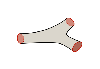
\includegraphics[height=2cm]{3pant.eps}
    \caption{A 3-pant}
  \end{center}
\end{figure}


\begin{theoreme}
In a 3-pant, we can compute the shortest 1-cut \textbf{homotopic} to a a boundary of the pant in O(Vlog(V)).
\end{theoreme}
\textit{Proof}:~~ \\
To establish this result, we need (see proof in: \cite{EricCours})
\begin{lemma}
In a cylinder, we can compute the shortest 1-cut homotopic to a a boundary of the cylinder in O(Vlog(V))
\end{lemma}
We can use this lemma on a 3-pant by cutting along a shortest path from the two remaining boundaries.
\fin

In \cite{EricLazarus}, one can find the following result:
\begin{lemma}
We can compute a first 3-pants decomposition \P$_0$ (a set of disjoint 1-cuts cutting \S{} into 3-pants) in O(gV).
\end{lemma}

Then we can give the pant optimization algorithm: compute a pants decomposition and optimize locally every boundary of a pant, until no improvement is possible.

\cite{EricLazarus} gives an upper bound for the number of iterations of this algorithm: the (difficult) proof uses rewriting on \textit{crossing words}, words encoding crosses between curves. \\
In particular, this algorithm is polynomial in its input. \\
\cite{EricLazarus} also proves that this algorithm is optimal, in this sense: each cut in the resulting pants decomposition \P{} is the shortest cut homotopic to the initial corresponding cut in \P$_0$. However this algorithm doesn't solve \PbOne: the homotopy classes of \P{} are not, \textit{a priori}, equal to the homotopy classes of a minimum system of 1-cuts (it is worth reminding that homotopy classes can't change while optimizing, with this algorithm).

\subsection{First attempts to a volume cutting}
A first idea, suggested before the internship, is to put volumical information on the surface.
\begin{defi}
The medial axis (or skeleton) of \S{} is the set of all points (different from \S{}) having more than one closest point on the object's boundary, i.e the centers of the open balls tangent to this boundary in at least two points.
\end{defi}
\begin{defi}
The local feature size is the distance to the medial axis.
\end{defi}
The method consists in defining the length of an edge as the product of the local feature size of the adjacent vertices and the Euclidean length of this edge. It is an estimation of the area that will be introduced if we are correcting an $\alpha$-junction using this edge. Then we can use a method from the previous section to compute an approximation of the shortest system of 1-cuts. However this not use all the volumic information and incoherent cuttings may happen.%[http://wiki.jmfavreau.info/post-doc_2009/projects/volumic_correction/report_june_2010]
\begin{figure}[h]
  \begin{center}
    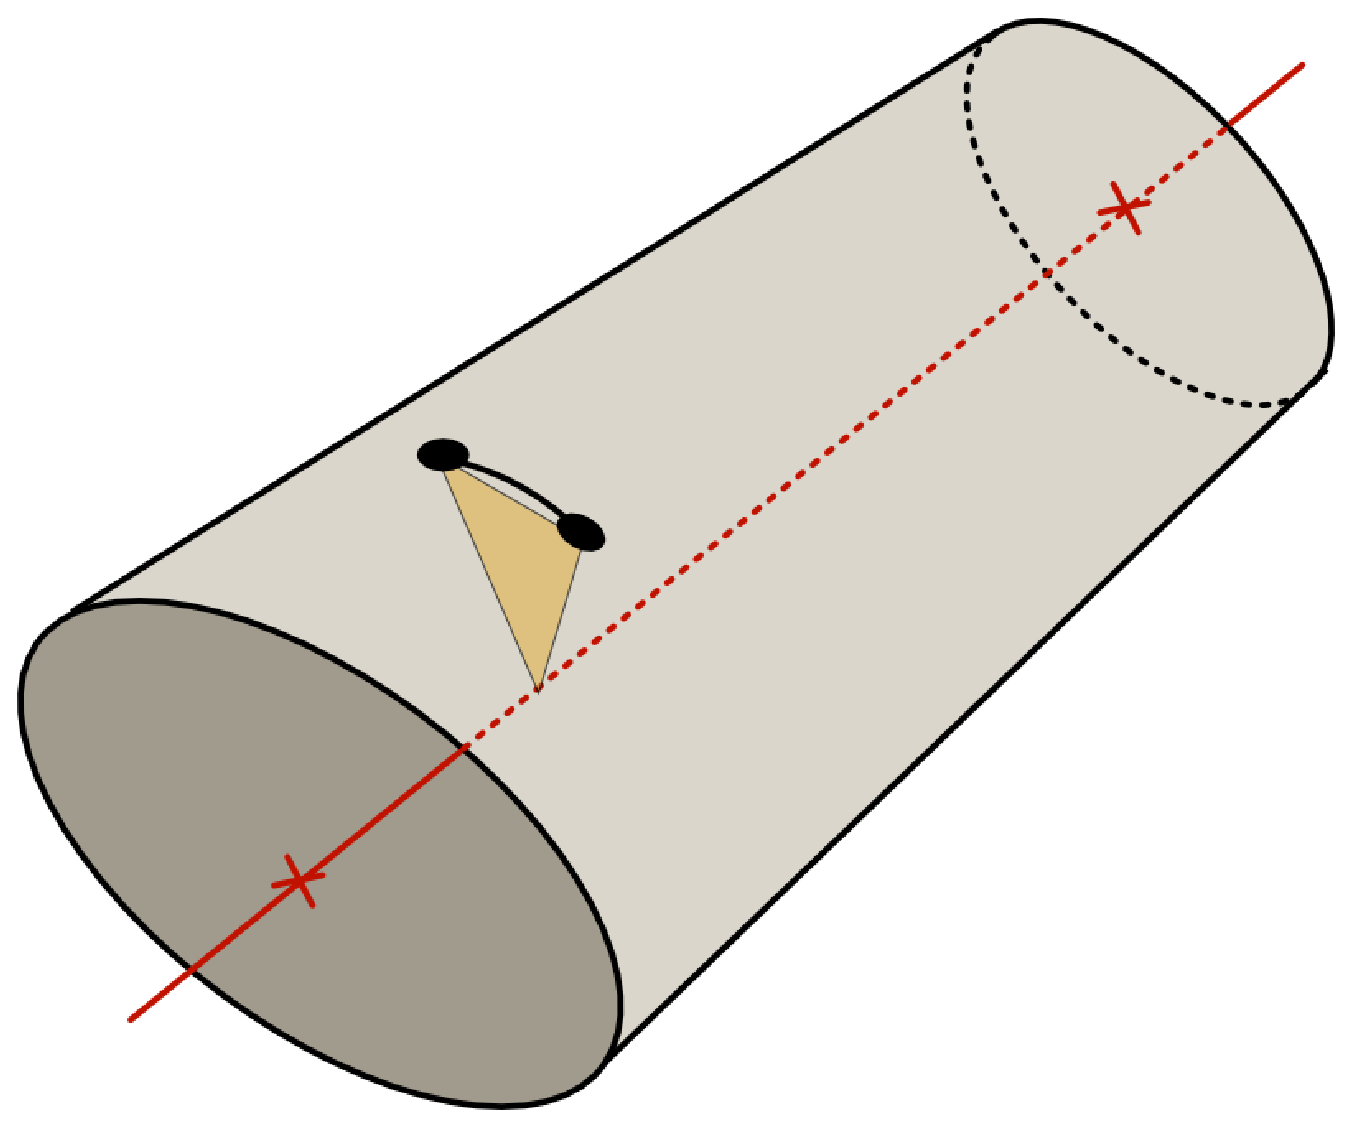
\includegraphics[height=2cm]{LFS.eps}
    \caption{Local feature size}
  \end{center}
\end{figure}

Another idea, inspired by the second above algorithm, is to decompose a volume into volumic 3-pants and to optimize them. It is the main idea of the approach described next.

\section{General algorithm}
\subsection{Overview}
The generic algorithm is the following:
\begin{itemize}
\item Compute a first volumic pants decomposition. 
\item Optimize (i.e change the location while decrasing the weight) every boundary of the cuts while possible.
\item Among the resulting pants decomposition, select a system of 2-cuts.
\end{itemize}
Two algorithms result from this pattern, which I call \textit{multi pants (MPA)} and \textit{single pant (SPA) algorithms}.
\subsection{First decomposition}
To compute a first cutting, I already described the cut locus method: given a set of points A, the \textit{A-cut locus} is the set of all points having more than one shortest path from A. \\
In the SPA, we simply choose an arbitrary point p, compute the p-cut locus \Sys{} and take as an initial decomposition the n-pant which boundaries are the g connected components of \Sys. \\
However, one may try to act more \textit{locally} and to use \textit{topological information} to guide the choice of the cuts (i.e to have an initial set of cuts close to the optimal) by decomposing the volume into many pants.  \\
For that purpose, the MPA first compute the skeleton (or medial axis) \K{} of the surface, using for example an \textit{erosion} process, see \cite{Cornea07} for a comprehensive survey of skeleton computation.\\
\begin{figure}[h]
\begin{center}
\begin{minipage}{0.4\linewidth}
\centering 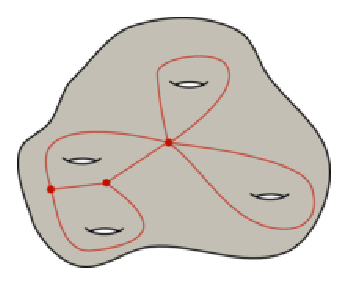
\includegraphics[height=3cm]{skeleton.eps}
\end{minipage}
\hfill
\begin{minipage}{0.4\linewidth}
\centering 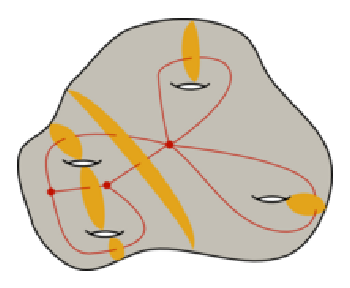
\includegraphics[height=3cm]{cutlocus_skeleton.eps}
\end{minipage}
\caption{Left: Skeleton. 
Right: Cuts associated to this skeleton. }
\end{center}
\end{figure}
Let B be the set of all intersection points of \K: the MPA basically compute the B-cut locus and use its connected components as a pants decomposition. \\
All the resulting pants need not have the same number of boundaries, but assuming that it is the case, we can know precisely the number of such pants:
\begin{theoreme}
Let p be the number of pants and c the number of cycles of any n-pant decomposition of \S{}.\\
Then p = 2(g-1) and c = 3(g-1).
\end{theoreme}
\textit{Proof}:~~ \\
For one pant P, according to Euler's formula: $V_P - E_P + F_P$ = 2 - b = - 1.\\
Since every couple of pants share a number of vertices equals to the number of edges shared, the number of pants is: $\sum_{P pant} (-V_P + E_P - F_P)$ = $V - E + F$ = 2 - 2g. \\
If we duplicate every pant we find 2c = 3g, since every cut has exactly two adjacent pants.
\fin

However, we can have intersections in this cut locus, and we are not sure to get 2-cuts [figure]. \\
\subsection{Pant(s) optimization}
I will first discuss how to optimize a single 2-cut, the next subsection will deal with the problem of selecting a cut to optimize. \\
We need to distinguish one kind of 2-cut:
\begin{defi}
A 2-cut \C{} is an auto 2-cut if the two pants adjacent to \C{} are actually the same pant. \\
\end{defi}

Since the SPA deals with only one pant, every 2-cuts are auto, and I first describe the optimization of an auto 2-cut \C, associated to a pant \P. \\
\subsubsection{Optimization of an auto 2-cut \C}
We first build the network N from \Dual{} the following way:
\begin{itemize}
\item Add two vertices s and t to \Dual{}.
\item Link s to all the vertices adjacent to \C{} on one side and the vertices adjacent to \C{} on the other side to t.
\item For each boundary \C' of \P{} delete \C', and if \C' $\neq$ \C{}, delete the edges with an end point adjacent to \C'{}.
\end{itemize}
The second part of this last point is needed in order to avoid intersections between 2-cuts. \\
Then, we compute a max flow on N (using Ford Fulkerson or Push-Relabel algorithm, for example) and we use the min cut - max flow theorem (the reader not familiar with flows on network may first read \cite{Cormen90}) to deduce a min \textit{\C s-t cut} (i.e, a min cut obtained by computing a max flow on \C) \MinC.
However, \MinC{} is not necessarly a 2-cut, for example \D{\MinC} is not necessarily connected, but in most applications we hope that \MinC{} is indeed a 2-cut, and from now on, \textbf{we assume that every min cut computed this way is a 2-cut}. \\ 
It is easy to see that, throughout the SPA, the pant structure is kept ((\Sys - \C) $\cup$ \MinC{} is a system of 2-cuts). \\
Moreover, the result of the SPA is likely to be, in practice, independant from the initial set of cuts. \\

However, it is possible that the best cut \MinC' intersects \C, and a max flow will not take it into account. \\
To avoid this problem, I suggested to take a \MinC{} s-t cut as a new cut, which correctness is validated by the theorem: \\
\begin{theoreme}
\MinC' doesn't intersect \MinC. 
\end{theoreme}
\textit{Proof}:~~ \\
\fin

\subsubsection{Optimization of a 2-cut \C{} (not auto)}
\begin{figure}[h]
  \begin{center}
    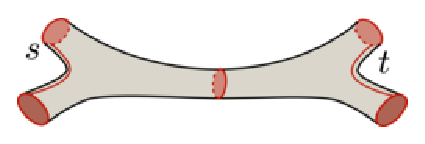
\includegraphics[height=1.4cm]{mincut.eps}
    \caption{Optimization of a cut}
  \end{center}
\end{figure}
Now we assume that \C{} is adjacent to two different pants \P$_1$ and \P$_2$, let \C$_{i, j}$ be the boundaries of \P$_i$ different from \C. \\
We need to be careful since we want to avoid non connected min cut [fig]. \\
We build N from \Dual the following way:
\begin{itemize}
\item Find a shortest tree $\mathcal{T}_{1}$ (resp. $\mathcal{T}_{2}$) connecting $\bigcup$\C$_{1, j}$ (resp. $\bigcup$\C$_{2, j}$). 
\item Link s to \C$_{1, j}$ and $\mathcal{T}_{1}$ and link \C$_{2, j}$ and $\mathcal{T}_{2}$ to t.
\end{itemize}
This way, every s-t cut is homotopic to \C: \textbf{we don't change homotopy classes}.
\subsection{Processing choice} 
Since every optimization of a 2-cut decreases the weight of the 2-cut system \Sys, and as there are only finitely many possible total weights (for a discrete volume), our algorithms are \textit{terminating}. \\
However, the final weight of \Sys{} and the complexity these algorithms depends crucially on the order we choose cuts to optimize. [fig] \\
Several possible choice were considered:
\begin{itemize}
\item Randomly.
\item Maximum weighted 2-cut first.
\item (All-Min) I also suggested, espcially in the SPA, to optimize the 2-cut \C{} which lead to the minimum possible \MinC, and we never optimize \MinC.
\item Optimize the 2-cut \C{} maximizing weight(\C) - weight(\MinC).
\end{itemize}
Bounding the number of iteration required for the 2 first points is likely to be very difficult (personal communication with �. Colin de Verdi�re). \\
However the All-Min choice requires $\Omega$(g$^2$) max flow, with the SPA: at the beginning there are g 2-cuts to optimize, so we compute g max flow, then we fix one 2-cut so we compute g - 1 max flow, and so on. \\
And indeed, g + g - 1 + $\ldots$ + 1 = $\frac{g(g+1)}{2}$ = $\Omega$(g$^2$). \\
Moreover, the validity of the All-Min choice is validated by:
\begin{theoreme}
Let \C$_1$, $\ldots$, \C$_k$ be the first k 2-cuts chosen by All-Min \\
C$_k$ is the minimum [non separating of the decoupage]2-Cut among all cuts not intersecting
\end{theoreme}
\textit{Proof}:~~ \\
Let ... Montrer que il existe cut tel que max flow le donne.
\fin

\subsection{Selection of a cutting system}
Proof that we get a topological ball.

\section{Improvements}
\subsection{Neighborhood}
%\textbf{We assume that all the capacities of the edges in \Dual{} are equal to one} (this is the case, for example, if \V{}  is a set of voxels and that we put a capacity on every edge equal to the area of the corresponding face).

The most time consuming part of both SPA and MPA being the computation of a max flow, one may try to improve its time complexity, and indeed, we can act more locally (for the importance of local search and neighborhood, see \cite{Papa98}). \\
The basic idea of the neighborhood algorithm is that, during Ford Fulkerson algorithm, we can select an augmentating path "near" the previous found paths, which restricts the number of edges to visit. To define precisely what the "near" means, we need a more dense graph:
\begin{defi}
The dual-adjacency graph \DualAdj{} is the graph with the same vertices as \Dual{} and with an edge (with neither a weight nor a capacity) between two vertices if the two corresponding volumic elements share at least one vertex.
\end{defi}
We need it to take into account path such as [fig].
\begin{defi}
If v is a vertex and p a set of vertices (for example, a path), d(v, p) (and d(p, v)) is the minimal length of a shortest path, in \DualAdj{}, between v and a vertex of p. \\
Given two set of vertices p and p', d(p, p') = max$_{v \in p}$ d(v, p'). \\
The p-neighborhood \N{p} is the set of all vertices v such that d(v, p) $\leqslant$ 1. \\
%If \Path{} = $\lbrace p_1, \ldots, p_n \rbrace$ is a set of paths, \N{\Path} = $\Delta$ \N{$p_i$} ( = ($\bigcup$  \N{$p_i$}) -  $\bigcup p_i$), and we define similarly \Ns{\Path}.
\end{defi}
\begin{rem}
d is a distance: d(p, p') = d(p', p), d(p, p') = 0 $\Longleftrightarrow$ p = p' and d(p, p'') $\leqslant$ d(p, p') + d(p', p''). \\
Moreover, a path p' $\in$ \N{p} if and only if d(p, p') $\leqslant$ 1.
\end{rem}

Then, to compute a max flow, we can use the following algorithm, which I call neighborhood algorithm: \\ 
\begin{algorithm}
\Path $\leftarrow$ shortest path from s to t in R (using BFS) \;
\While{There is an augmenting path p from s to t in R $\cap$ \Ns{\Path}}
{
	Augment flow along p. \;
	\Path $\leftarrow$ \Path $\cup$ p \;
}
\end{algorithm} \\

Of course, the first path computed may visit all the reachable edges (as in the classic Ford Fulkerson), but all other paths are searched in the growing neighborhood. \\
The following theorem shows that we actually get a max flow at the end of the neighborhood algorithm:
\begin{theoreme}
Assume we are computing a max flow in \V, using neighborhood algorithm and that we already found n (n $\geqslant$ 1) augmenting paths \Path = $\lbrace p_1, \ldots, p_n \rbrace$. \\
Let R be the residual network, and f the current flow. \\
If there is no path from s to t in R $\cap$ \N{\Path} then f is a max flow.
\end{theoreme}
\textit{Proof}:~~ \\
Assume f is not a max flow: there is at least one path p$_0$ from s to t in R. \\
$\lbrace$ d(p, \Path), p path from s to t in R $\rbrace$ is a finite, non empty (p$_0$ belongs to it) set of $\mathbb{N}$ so it has a minimum m, let p$_1$ be a path such that d(p$_1$, \Path) = m. \\
If m $\leqslant$ 1, p$_1$ $\in$ R $\cap$ \N{\Path} and the theorem is proved. \\
Otherwise, let v be a vertex in p$_1$ such that d(v, \Path) $\geqslant$ 2.\\
Since d(v, \Path) $\geqslant$ 2, \N{\Path} $\cap$ \N{v} = $\varnothing$, and every edge in \N{v} has a flow equal to 0 (i.e, these edges are in the residual graph R). \\
Let q be the path \N{v} $\cap$ p$_0$. \\
Since all paths from s to t are homotopic (such that there is no "hole" between them), we can find a path q' in \N{v} with same extremities than q and replace q by q' such that for all vertices w added this way, d(w, \Path) $<$ d(v, \Path). \\
If we do this with all such vertex v, we create a path p such that d(p, \Path) $<$ m, a contradiction. So m $\leqslant$ 1.
\fin

\begin{rem}
If we allow capacities to be different, we have the following weaker statement: if there is no path from s to t in R $\cap$ \N{\Path} then f is a max flow. 
\end{rem}


\subsection{Processing order and intersections}
\subsection{Complexity}

\section{Implementation}
\subsection{Overview}
Initially, it was planned that I develop the optimization part of the MPA, and that the rest of the team will develop the initial pants decomposition, all in C++. \\
After two weeks working on the core algorithm, I decided to use tetrahedra, although more complicated to implement than voxels, to be able to work on surfaces, on Blender for example and use TetGen to tetrahedralize them. \\ 
I also used TetMeshLib, a library to manage tetrahedral meshes that Marco Attene developed. \\
To both automatize the different tools of the algorithm and visualize more easily, I wrote a script in Blender Python API. \\
At the end of the internship, I worked together with Jean Marie Favreau, using GitHub. \\
Globally, I wrote about 3000 lines in C++ and 400 in Python and the documentation, built with doxygen, is available at [url]. \\

\subsection{SGL}
SGL relies on \textit{generic programming}: an ADT (Abstract Data Type) defines the required methods and semantic for a class and is used through template parameter. \\
For example, the class BFS (Breadth First Search) has a Graph template parameter, which must provide, among other, a class named iterator giving a way to iterate over all edges adjacent to a given vertex. \\
OC3D was designed in a similar way. \\

\subsection{Data structures}
\begin{figure}[h]
\begin{center}
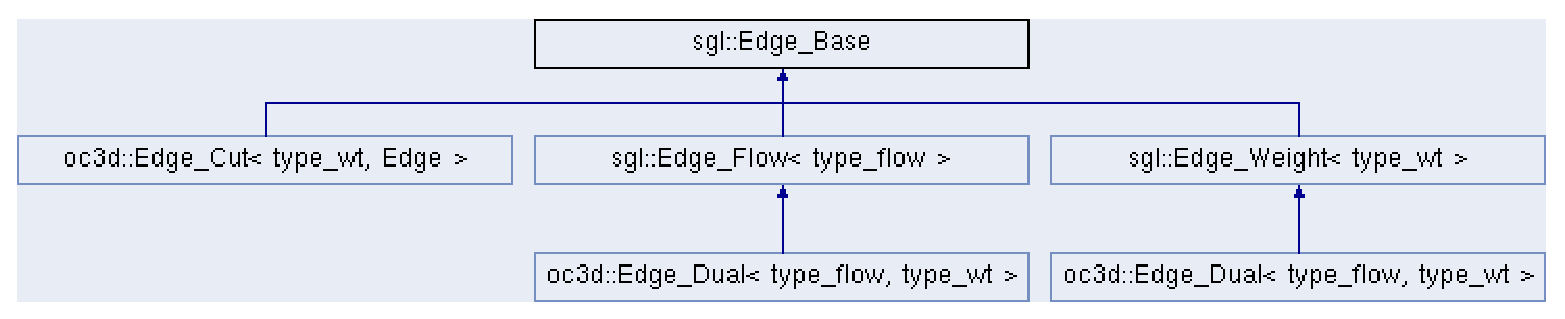
\includegraphics[height=2.4cm]{edges.eps}
\caption{Hierarchy of edge classes (an arrow means "inherits from")}
\end{center}
\end{figure}
Since we often need to iterate over all edges adjacent to a vertex, every graph is implemented as a adjacency list graph (\verb!Graph_List<Edge>!). \\
I use mainly three graphs: the pants graph, the dual graph \Dual{} and the dual-adjacency graph \DualAdj. \\
The pants graph is directed, while \Dual{} and \DualAdj{} are undirected, this is needed by the way the residual graph is used by the implementation of Ford Fulkerson algorithm: we access the residual capacity of an edge of \Dual{} (of type \verb!Edge_Dual!) providing the direction of the edge (i.e, the end extremity), it uses less memory and time since we manipulate only one edge pointer (this edge pointer is stored in the adjacency list of both extremities). \\
Since the network we use for Ford Fulkerson algorithm is not oriented, every edge of \Dual{} has a reverse (in the opposite direction) and every edge has a pointer to its reverse. \\ 
An edge (i.e, a 2-Cut) of the pants graph is of type \verb!Edge_Cut!:  its extremities are the pants adjacent to the corresponding 2-Cut and it stores the list of the pointers to \verb!Edge_Dual! elements included in the 2-Cut. \\
Every \verb!Edge_Dual! in a \verb!Edge_Cut! has the same orientation, i.e their end extremities are in the same pant. \\
This is needed to know to which vertices we must link the source (or sink) before running Ford Fulkerson algorithm, or to delete the edges out of the pant we optimize (subsection \ref{orientation} explains how to orientate a cut). \\
To avoid time waste, every 2-Cut has a reverse and a pointer to it.

\subsection{Core algorithm}
\begin{figure}[h]
\begin{center}
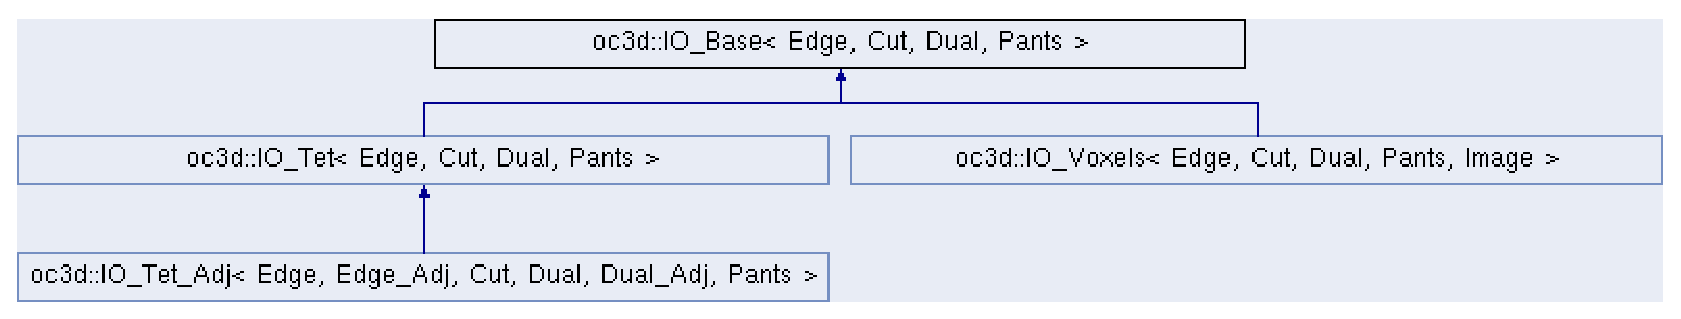
\includegraphics[height=2.4cm]{IO.eps}
\caption{Hierarchy of IO classes.}
\end{center}
\end{figure}
To improve genericity, the algorithm first construct the dual graph (which depends on the the representation used - voxels or tetrahedra) and then works only on the dual graph. \\
For that purpose, an object is used to deal with representation-dependant operations, IO\_Base implements the required methods of such an object but the dual graph must be set manually, IO\_Tet defines how to make the dual graph from tetrahedra and IO\_Voxels from voxels image. \\
IO\_Tet\_Adj also defines how to build the adjacency-list graph.

After the dual graph is made, we can search a max flow on it with a class derived from \verb!Max_Flow!, and \verb!Cut_vertices! is a class giving a min cut from a max flow, searching for the set S of every vertices reachable from the source s and setting as the cut the set of edges connecting S and S$^c$.
\begin{figure}[h]
\begin{center}
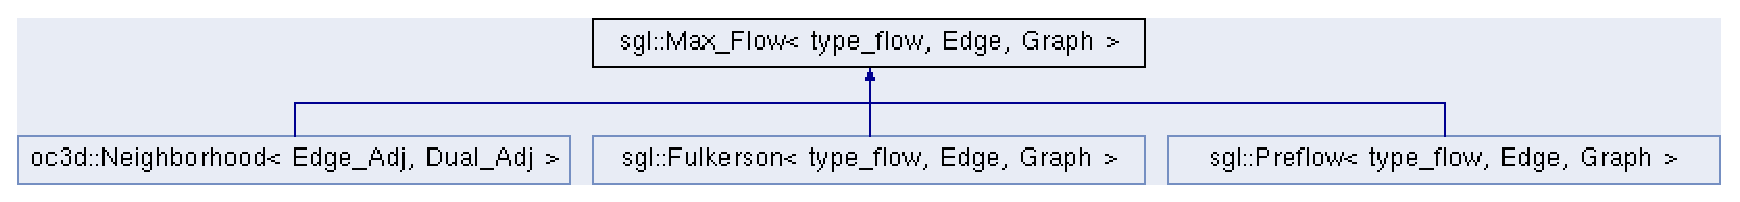
\includegraphics[height=1.4cm]{Max_Flow_.eps}
\caption{Simplified hierarchy of max flow classes. }
\end{center}
\end{figure}
\subsection{Orientation} \label{orientation}
When we get a cut, selecting it with Blender for example, we must orientate it. \\
After discussing it with Jean Marie Favreau and Vincent Barra, the best solution may be the following: \\
\begin{itemize}
\item Take an element of the cut (a triangle or a square, say a triangle abc), give an orientation to it, which can be viewed as a permutation $\sigma$ of its vertices.
\item For each triangle uvw adjacent to it with an edge uv, if $\sigma(u)$ = v,  defines the orientation on t according to the permutation vuw.
\item Repeat the second point replacing abc by all new triangles with an orientation, until every triangle has an orientation.
\item For each edge uv in the cut, associated to a triangle with orientation (abc), compute det(a,b,c): if it is negative, replace uv by vu. 
\end{itemize}
This algorithm is clearly linear (assuming that the number of vertices of an element of a cut is fixed).
\begin{figure}[h]
\begin{center}
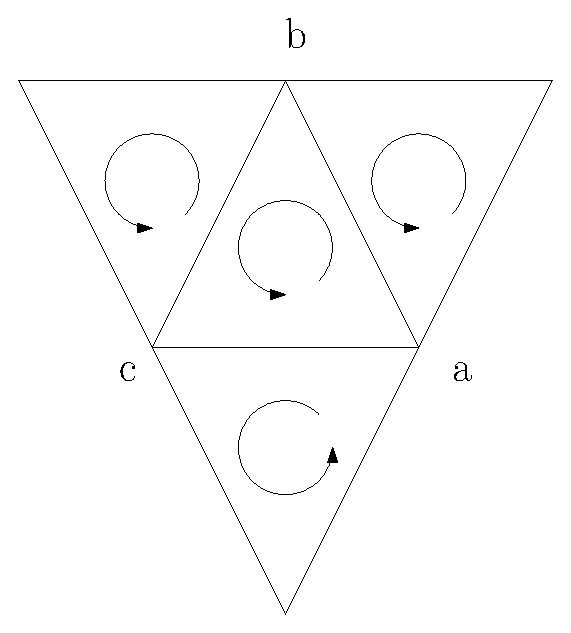
\includegraphics[height=4cm]{orientation.eps}
\caption{An orientation.}
\end{center}
\end{figure}

\subsection{Python script}
The script (which can be found together with a video describing its working) I wrote for Blender uses, with pipeline,  OC3D\_debug, a command-line debugger which can, among other, load a mesh, make the dual graph, optimize cuts step by step and output various information. \\
To avoid freezing Blender while optimizing a cut I used several threads and I had to synchronize the threads, OC3D\_debug and TetGen.
\begin{figure}[h]
\begin{center}
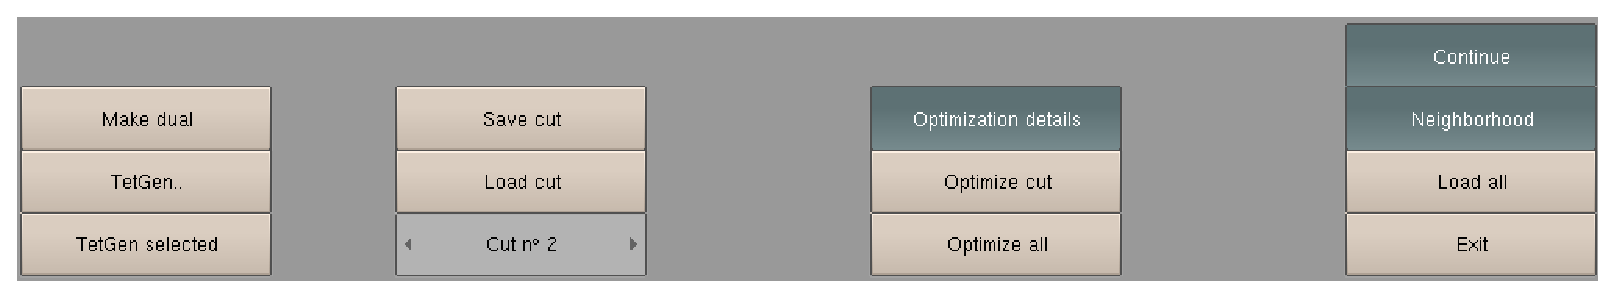
\includegraphics[height=2.3cm]{ex_script_.eps}
\caption{Blender Python API interface.}
\end{center}
\end{figure}


\subsection{Running time comparison}
To compare the algorithms of max flow, I tested them on a slighty modified torus, with various number of vertices. \\
The examples can be found at : [url]. \\
The timing runs were performedon a Dell inspiron 1520 with and Intel Core 2 Duo T7300 Processor (2.0GHz, 4MB L2 cache) and 2048 Mo memory. \\
Compilation was done with Visual C++ 2008 with all optimization flags set for maximum speed. \\
The times require by the continue neighborhood algorithm is of same order of the time required by TetGen which has  the complexity O(\S$^2$) required by Delaunay tetrahedrization (about 80 seconds for the torus which dual has a complexity 1750000), see \cite{TetGen}.

\begin{table}[htbp]
\begin{center}
\begin{tabular}{|c|c|c|c|}
\hline
Complexity (edges + vertices) of the dual graph & Classic & Neighborhood & Continue \\ \hline
200K & 111s & 61s & 29s \\ \hline
900K & 1147s & 236s & 101s \\ \hline
1750K & 2975s & 318s & 158s \\ \hline
\end{tabular}
\end{center}
\label{time}
\caption{Running time in seconds of the optimization of one 2-Cut using several algorithms of max flow (K stands for 1000).}
\end{table}

The advantage of a neighborhood increases significantly as the number of vertices of \Dual{} increases. \\
I also compared, on the dual graph with complexity 900000, the time required for a BFS at different moments of the algorithms. \\
I split the execution of the algorithms in different steps defined by the augmentation of the neighborhood used by the continue neighborhood algorithm (thus, the continue neighborhood algorithm found 1 path before augmentating, then 21, 129 and so on). \\
Then I compared the number of edges of the neighborhood in which the paths were found, the total time during the step, and the average (shortened Avg) time of a BFS. \\
The advantage of a neighborhood decreases slighty during the algorithm, since the neighborhood increases as the number of edges visited by a BFS on the whole graph decreases (some edges have then zero capacity and disappear from the residual graph), so the algorithm is likely to be more efficient if the min cut is small (this is especially true for voxels with capacity one, since the number of iterations is directly the number of iterations of the algorithm).
\begin{table}[h]
\footnotesize{
\begin{center}
\begin{tabular}{|c|c|c|c|c|c|c|c|c|}
\hline
 & \multicolumn{ 3}{c|}{Continue neighborhood} & \multicolumn{ 3}{c|}{Neighborhood} & \multicolumn{ 2}{c|}{Classic} \\ \hline
Paths found & Edges & Total time & Avg time & Edges & Total time & Avg time & Total time & Avg time \\ \hline
1 & 101 (in path) & 250 & 250 & 101 (in path) & 250 & 250 & 250 & 250 \\ \hline
21 & 2452 & 41 & 1,95 & 2452 & 49 & 2,33 & 4917 & 234,14 \\ \hline
129 & 4240 & 283 & 2,19 & 5084 & 446 & 3,46 & 30140 & 233,64 \\ \hline
363 & 9428 & 1295 & 3,57 & 11282 & 2500 & 6,89 & 86221 & 237,52 \\ \hline
741 & 21822 & 5234 & 7,06 & 25930 & 10028 & 13,53 & 165232 & 222,99 \\ \hline
1735 & 44944 & 22627 & 13,04 & 50886 & 46345 & 26,71 & 364113 & 209,86 \\ \hline
2798 & 87172 & 66810 & 23,88 & 101262 & 144944 & 51,8 & 559327 & 199,9 \\ \hline
249 & 161664 & 10568 & 42,44 & 184092 & 16781 & 67,39 & 48611 & 195,22 \\ \hline
0 & 173368 & 22 & 22 & 189654 & 33 & 33 & 94 & 94 \\ \hline
\end{tabular}
\end{center}
\label{}
\caption{Detailed time comparison}
}
\end{table}
I didn't have the time to test this algorithm on voxels, but for non degenerated volume, the first neighborhood will be at most eight times the length of the first path found (if the path is a straight path, there is exactly eight disjoint paths adjacent to it. \\
For that example, it means that the first neighborhood is likely be about 800 edges instead of 2452 for tetrahedra, three times less. \\
Then I expect the neighborhood algorithm to be more efficient with voxels.

\begin{figure}[h]
\begin{center}
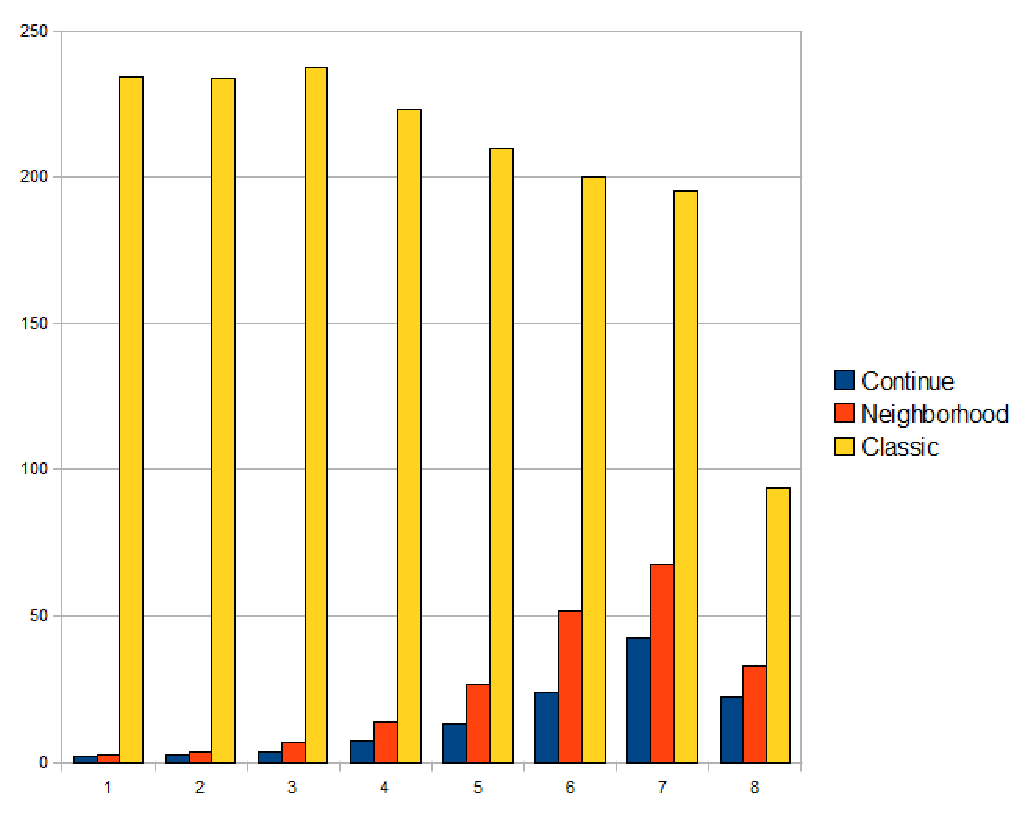
\includegraphics[height=6.cm]{diagram_time.eps}
\caption{Average time of a BFS with respect to the step in the CNA.}
\end{center}
\end{figure}
\section{Conclusion}
Integrated to FAST project.
\section{Appendix}
\subsection{Mathematical background}
\begin{defi}
is a continuous map \L{} : [0, 1] $\longrightarrow$ \S{} such that \L(0) = \L(1)
\end{defi}
Warning: non separating neq contractible

\subsection{Applications}
\subsection{SGL}

\begin{small}
\begin{thebibliography}{1}
\bibitem{JMThese} J.-M. Favreau. Outils pour le pavage de surfaces. PhD thesis, Blaise Pascal university, 2009.
\bibitem{EricThese} �. Colin de Verdi�re. Raccourcissement de courbes et d�composition de surfaces. PhD thesis, Paris 7 university, 2003.
\bibitem{EricLazarus} �. Colin de Verdi�re and F. Lazarus. Optimal pants decompositions and
shortest homotopic cycles on an orientable surface. Proceedings of the 11th Symposium on Graph Drawing , 2003.
\bibitem{Favreau09} J.-M. Favreau, V. Barra. Conformal Flattening of the Cortical Surface using a Topological and Geometrical Cutting. SEECCM, South-East European Conference on Computational Mechanics, Island of Rhodes, Greece, 2009.
\bibitem{EricCours} �. Colin de Verdi�re. Algorithms for graphs on surfaces, M.P.R.I. course Master 2. 2009-2010.
\bibitem{FAST} Cortical surface mapping using topology correction, partial flattening and 3D shape context-based non-rigid registration for use in quantifying atrophy in Alzheimer's Disease. Preprint submitted to International Journal of Biomedical Imaging, March 2010.
\bibitem{Erickson02} J. Erickson, S. Har-Peledz. Optimally Cutting a Surface into a Disk. Discrete and Computational Geometry, July 2, 2002.
\bibitem{Cornea07} N. D. Cornea, D. Silver, P. Min. Curve skeleton properties, applications and algorithms. IEEE Transactions on Visualization and Computer Graphics 13 (2007), pp 530-548.
\bibitem{Cormen90} T. Cormen, C. Leiserson, R. Rivest. Introduction to algorithms. MIT Press, 1990.
\bibitem{Diestel02} R. Diestel. Graph Theory, volume 173 of Graduate Texts in Mathematics. Springer-Verlag, 2000.
\bibitem{Papa98} C. H. Papadimitriou, K. Steiglitz. Combinatorial optimization: Algorithms and Complexity. Dover Publications, 1998.
\bibitem{TetGen} H. Si. TetGen: User's manual. 2006.
\end{thebibliography}
\end{small}

\textit{Proof}:~~ \\
\fin
\end{document}